\documentclass[letterpaper,11pt]{article}
\usepackage{graphicx}
\usepackage{listings}
\usepackage[super]{nth}

\lstset{
	basicstyle=\footnotesize,
	breaklines=true,
}

\begin{document}

\begin{titlepage}

\begin{center}

\Huge{Assignment 2}

\Large{CS 595:  Introduction to Web Science}

\Large{Fall 2013}

\Large{Shawn M. Jones}

\Large Finished on \today

\end{center}

\end{titlepage}

\newpage
\section*{1}

\subsection*{Question}

\begin{verbatim}
Write a Python program that extracts 1000 unique links from
Twitter.  You might want to take a look at:

http://thomassileo.com/blog/2013/01/25/using-twitter-rest-api-v1-dot-1-with-python/

But there are many other similar resources available on the web.  Note
that only Twitter API 1.1 is currently available; version 1 code will
no longer work.

Also note that you need to verify that the final target URI (i.e., the
one that responds with a 200) is unique.  You could have different
shortened URIs for www.cnn.com.

You might want to use the search feature to find URIs, or you can
pull them from the feed of someone famous (e.g., Tim O'Reilly).

Hold on to this collection -- we'll use it later throughout the semester.
\end{verbatim}

\newpage
\subsection*{Answer}

Extracting 1000 unique links from Twitter was a more complex endeavor than expected.

It required the use of 4 distinct scripts run in the following order:
\begin{enumerate}
\item \verb+gimmetweets.py+ \textless starting tweet id\textgreater \textless tweet count per call\textgreater \textless \# of api calls \textgreater \textless screen name\textgreater
	\begin{itemize}
	\item Starts at a given tweet ID and works backward, printing out all tweets for the given screen name, making only a certain number of api calls to ensure Twitter does not lock out the application.
	\item The intention is to run this once for each screen name for which we want to gather tweets, then pass the output to a file via redirection ('\verb+>+')
	\end{itemize}
\item \verb+extractURIsFromTweets.py+ \textless filename \#1 containing tweets\textgreater \textless filename \#2... \textgreater
	\begin{itemize}
	\item Runs through all of the tweets, extracting URIs that match a simple URI pattern of \verb+"http://[\S]*"+
	\item Each URI is dereferenced, passing through all redirects.  If a status code of 200 comes back, the URI is saved for the next step.
	\end{itemize}
\item \verb+combineLists.py+ \textless filename \#1 containing uris\textgreater \textless filename \#2... \textgreater
	\begin{itemize}
	\item Combine all of the files gathered together in the last step, sort the entries, and eliminate duplicates.
	\end{itemize}
\item \verb+extractRandom1000Links.py+ \textless input file containing links\textgreater
	\begin{itemize}
	\item Because more than 1000 links were acquired, this script randomly generates a representative sample of 1000 links form the file generated in the last step, preventing needless hours processing more than 1000 links in the rest of this assignment.
	\end{itemize}
\end{enumerate}

The 4 scripts allowed resumption of processing if an error state was encountered at any point.  For example, \verb+gimmetweets.py+ could be cut off because it reached Twitter's hourly request limit\cite{twitter}.  Because it was time consuming (in minutes, sometimes hours) to complete some of these tasks, splitting the scripts up in this way allowed work to be saved across runs.  Even if there was some overlap, \verb+combineLists.py+ took care of any extra URIs that were processed repeatedly.

Early testing of the \emph{expanded\_url} field provided by the Twitter API showed that even though a URI was present in the tweet text, sometimes it did not appear as a value in \emph{expanded\_url}, so it was inconsistent.  To account for this, all tweets were extracted by \verb+gimmetweets.py+ and later processed with \verb+extractURIsFromTweets.py+.

The following screen names were followed for data:
\begin{itemize}
\item BarackObama - \nth{44} President of the United States
\item BillGates - Former Microsoft CEO, now attempting to rid the world of Malaria, in addition to other feats
\item CNN - original 24 hour news channel
\item GeorgeTakei - Former helmsman on Star Trek, now Internet celebrity
\item MaddowBlog - left leaning Rhodes Scholar political pundit Rachel Maddow
\item SethMacFarlane - writer and comedian, best known as the creator of the TV series \emph{Family Guy}
\item dailykos - faaaaar left leaning news source
\item nprnews - National Public Radio
\end{itemize}

In retrospect, I could have saved a lot of time with \verb+extractURIsFromTweets.py+ by using parallel execution.  The program could have broken a given list of tweets up and then executed against each sublist, combining the whole once all were done.

Parallel execution would have saved little for \verb+gimmetweets.py+ because of the number of requests limited by Twitter.

The list of URIs is available at:
https://github.com/shawnmjones/cs595-f13/blob/master/assignment2/work/q1/uris/urilist-final.txt

The following sections show the source code of each of these scripts.

\newpage
\paragraph{gimmetweets.py}\mbox{} \\

\lstinputlisting[language=Python,frame=single,caption={Python program for acquiring tweets for a given screen name}, label=lst:q1-1,captionpos=b,numbers=left,showspaces=false,showstringspaces=false,basicstyle=\footnotesize]{work/q1/gimmetweets.py}

\newpage
\paragraph{extractURIsFromTweets.py}\mbox{} \\

\lstinputlisting[language=Python,frame=single,caption={Python program for extracting URIs from a file of tweets}, label=lst:q1-2,captionpos=b,numbers=left,showspaces=false,showstringspaces=false,basicstyle=\footnotesize]{work/q1/extractURIsFromTweets.py}

\newpage
\paragraph{combineLists.py}\mbox{} \\

\lstinputlisting[language=Python,frame=single,caption={Python program for combining, sorting, and uniquing several files}, label=lst:q1-3,captionpos=b,numbers=left,showspaces=false,showstringspaces=false,basicstyle=\footnotesize]{work/q1/combineLists.py}

\newpage
\paragraph{extractRandom1000Links.py}\mbox{} \\

\lstinputlisting[language=Python,frame=single,caption={Python program for randomly extracting 1000 lines from a given file}, label=lst:q1-3,captionpos=b,numbers=left,showspaces=false,showstringspaces=false,basicstyle=\footnotesize]{work/q1/extractRandom1000Links.py}

\newpage
\section*{2}

\subsection*{Question}

Original:
\begin{verbatim}
Download the TimeMaps for each of the target URIs.  We'll use the ODU 
Memento Aggregator, so for example:

URI-R = http://www.cs.odu.edu/

URI-T = http://mementoproxy.cs.odu.edu/aggr/timemap/link/http://www.cs.odu.edu/

Create a histogram of URIs vs. number of Mementos (as computed from
the TimeMaps).  For example, 100 URIs with 0 Mementos, 300 URIs
with 1 Memento, 400 URIs with 2 Mementos, etc.
\end{verbatim}

\newpage
\subsection*{Answer}

\subsubsection*{The Data Collection}
The script \verb+countMementos.py+ acquires the TimeMap for each link from a file containing many links, then parses that TimeMap and counts the number of mementos present.  Requests that generate a 404 are recorded as having 0 mementos.  The mementos are counted using a regular expression.

Because the first run of this script took almost 10 hours to complete, I used the Unix \verb+split+ command to divide the 1000 links into 5 files of 200 links each, like so:
\begin{lstlisting}[frame=single]
split -l 200 ../../q1/uris/urilist-final.txt
\end{lstlisting}
which produced the files \verb+xaa+ through \verb+xae+.

I then ran the script against each file in turn.  Running these in parallel drastically reduced the run time.  In fact, the original 10 hour run was on Sunday afternoon.  The second run was on Monday night during dinner, which took 1 hour.

The script \verb+countMementos.py+ is run like so:
\begin{lstlisting}[frame=single]
./countMementos.py workspace/xae > xae.txt
\end{lstlisting}

The source code for doing the dereferencing and processing of each Time Map is shown in Listing \ref{lst:q2}.

Once the 5 files were acquired, they were combined together using the Unix \verb+cat+ command and stored in the file \verb+mementoCounts.txt+ like so:
\begin{lstlisting}[frame=single]
cat xaa.txt xab.txt xac.txt xad.txt xae.txt > mementoCounts.txt
\end{lstlisting}

\subsubsection*{The Results}

The histogram in Figure \ref{fig:q2histy1} on page \pageref{fig:q2histy1} is difficult to read.  This histogram was generated in R using buckets of size 1.  This was done to keep the y-axis low, because there are 375 URIs with 0 mementos and 244 URIs with 1 memento, totaling more than half of all data recorded.

Outliers also skew the results.  Two outliers have 22,157 and 10543 mementos.  Stripping out these outliers gets us to Figure \ref{fig:q2histy2} on page \pageref{fig:q2histy2}, which shows a slightly better visualization, but there is still such a jump between the low number of mementos to those at 3000 that it is still difficult to see a pattern.

If we focus on the highest number of records, mementos less than 100, the plot actually begins to look like a histogram in Figure \ref{fig:q2histy3} on page \pageref{fig:q2histy3}, and we can see the precipitous drop between 0 and 2, and the ``Long Tail'' decline thereafter.

\begin{figure}
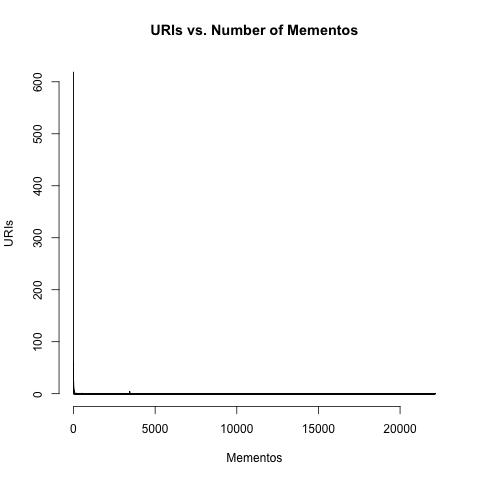
\includegraphics[scale=0.7]{work/q2/q2-histogram1.png}
\caption{Histogram of URIs vs. number of Mementos for the entire dataset (generated from code in Listing \ref{lst:q2R})}
\label{fig:q2histy1}
\end{figure}

\begin{figure}
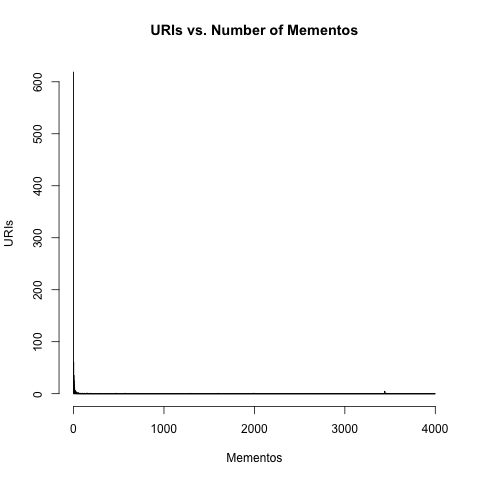
\includegraphics[scale=0.7]{work/q2/q2-histogram2.png}
\caption{Histogram of URIs vs. number of Mementos for URIs with less than 10,000 Mementos (generated from code in Listing \ref{lst:q2R})}
\label{fig:q2histy2}
\end{figure}

\begin{figure}
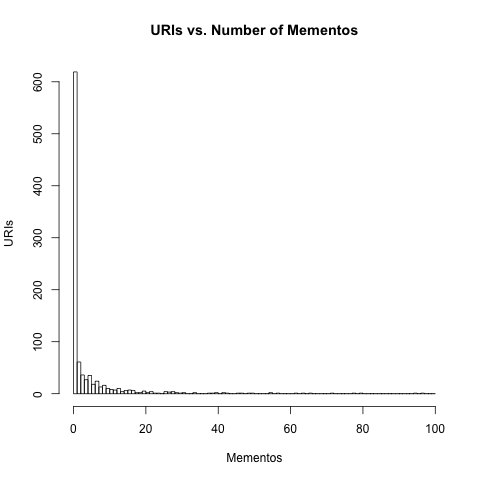
\includegraphics[scale=0.7]{work/q2/q2-histogram3.png}
\caption{Histogram of URIs vs. number of Mementos for URIs with less than 100 Mementos (generated from code in Listing \ref{lst:q2R})}
\label{fig:q2histy3}
\end{figure}


\newpage

\lstinputlisting[language=Python,frame=single,caption={Python program for processing Time Maps for a given file full of links}, label=lst:q2,captionpos=b,numbers=left,showspaces=false,showstringspaces=false,basicstyle=\footnotesize]{work/q2/countMementos.py}

\newpage
\lstinputlisting[language=R,frame=single,caption={R program for generating the histograms for Question 2}, label=lst:q2R,captionpos=b,numbers=left,showspaces=false,showstringspaces=false,basicstyle=\footnotesize]{work/q2/q2-histogram.R}

\newpage
\section*{3}

\subsection*{Question}

\begin{verbatim}
Estimate the age of each of the 1000 URIs using the "Carbon Date" tool:

http://ws-dl.blogspot.com/2013/04/2013-04-19-carbon-dating-web.html

Note: you'll have to download the tool and install; don't try to use the 
web service.  

For URIs that have > 0 Mementos and an estimated creation date,
create a graph with age (in days) on one axis and number of mementos
on the other.
\end{verbatim}

\newpage
\subsection*{Answer}

\subsubsection*{The Data Collection}
Since I did not have Python 2.6 readily available, I modified Carbon Date to work with Python 2.7 and shared it with the author so he could share with others.

From some test runs, it became apparent that the Carbon Date tool takes between 1 and 7 minutes to query all of its services for a given URI.  A worst case scenario yields:

\[
\frac{7 \textrm{ minutes}}{1 \textrm{ URI}} \times {1000 \textrm{ URIs}} = {7000 \textrm{ minutes}} \times \frac{1 \textrm{ day}}{1440 \textrm{ minutes}} \approx {5 \textrm{ days}}
\]

I modified the Carbon Date tool to accept a configuration file as an argument (also shared with the author), then ran it 5 times across 5 different screen sessions using 5 different configuration files containing 5 different port numbers.  I limited it to 5 due to the fact that the Bitly API, used by Carbon Date, does not allow more than 5 simultaneous connections\cite{bitly}.

Then I did the same for the Carbon Date tool client shown in Listing \ref{lst:q3Query}.

Here's an example run of the Carbon Date client using a subset of the 1000 links in a file named \verb+xae+.
\begin{lstlisting}[frame=single]
./queryCarbonDateFor1000Links.py http://ganesh:8547/cd xae > xae.data
\end{lstlisting}

Getting the dates was not enough, of course, because we need the ages in days.  Listing \ref{lst:q3Convert} takes in the list from the previous script and generates a tab-delimited file containing the URIs and ages in days.  It is run like so:
\begin{lstlisting}[frame=single]
./listAgesFromCdlist.py work/cdlist-final.txt > daycounts-final.txt
\end{lstlisting}

What we really want is to create a graph for all URIs that have \textgreater 0 Mementos and an estimated creation date.  This is where Listing \ref{lst:q3Join} comes in.  This script joins the tab-delimited file generated from Question 2 with the tab-delimited file containing our ages in days, eliminates those with 0 Mementos and no carbon dates, then generates another tab-delimited file that can be fed into R for our scatter plot.

This script is run like so:
\begin{lstlisting}[frame=single]
./joinAndProcessAgesWithMementoData.py ../q2/mementoCounts.txt daycounts-final.txt > mementosVsAge.txt
\end{lstlisting}

\subsubsection*{The Results}

Because, as shown in Figure \ref{fig:q2histy3}, the majority of the memento counts are between 0 and 2, most of the data points in Figure \ref{fig:q3scatter} are on the left side, with a large number of mementos being roughly less than 1200 days old.  There are also two outliers, our friends with 22,157 and 10543 mementos, who seem to be much older.  In a perfect world, the whole graph would follow the pattern of these two outliers, with the number of mementos increasing from the age of first creation.

One could make the argument that, because the majority of the URIs are ``young'' when cited, and it takes some time to get archived, that this graph may make sense, especially for twitter postings.  This theory doesn't quite fit, as there are URIs reaching far into the past (http://www.tietheknot.com from 1996?) with very few Mementos.  Twitter was founded in 2006\cite{laracinisomo}, so that places an lower bound on when these URIs would have originally been cited.

\begin{figure}
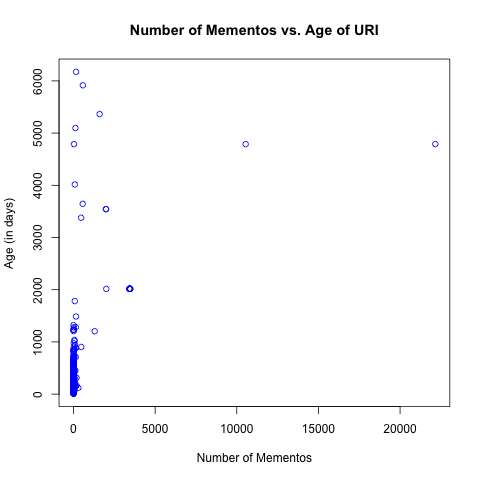
\includegraphics[scale=0.56]{work/q3/q3-scatterplot.png}
\caption{Number of Mementos vs. Age of URI (generated via code in Listing \ref{lst:q3R})}
\label{fig:q3scatter}
\end{figure}

\newpage
\lstinputlisting[language=Python,frame=single,caption={Python program for remotely querying the Carbon Date tool}, label=lst:q3Query,captionpos=b,numbers=left,showspaces=false,showstringspaces=false,basicstyle=\footnotesize]{work/q3/queryCarbonDateFor1000Links.py}

\newpage
\lstinputlisting[language=Python,frame=single,caption={Python program for calculating the ages based on dates gathered from the Carbon Date tool}, label=lst:q3Convert,captionpos=b,numbers=left,showspaces=false,showstringspaces=false,basicstyle=\footnotesize]{work/q3/listAgesFromCdlist.py}

\newpage
\lstinputlisting[language=Python,frame=single,caption={Python program for calculating the ages based on dates gathered from the Carbon Date tool}, label=lst:q3Join,captionpos=b,numbers=left,showspaces=false,showstringspaces=false,basicstyle=\footnotesize]{work/q3/joinAndProcessAgesWithMementoData.py}

\newpage
\lstinputlisting[language=R,frame=single,caption={R program for generating the scatterplot for Question 3}, label=lst:q3R,captionpos=b,numbers=left,showspaces=false,showstringspaces=false,basicstyle=\footnotesize]{work/q3/q3-scatterplot.R}

\newpage
\bibliographystyle{acm}
\bibliography{references}

\end{document}